\appendix

\chapter{Diagrama de Classes completo}

\begin{figure}
\centering
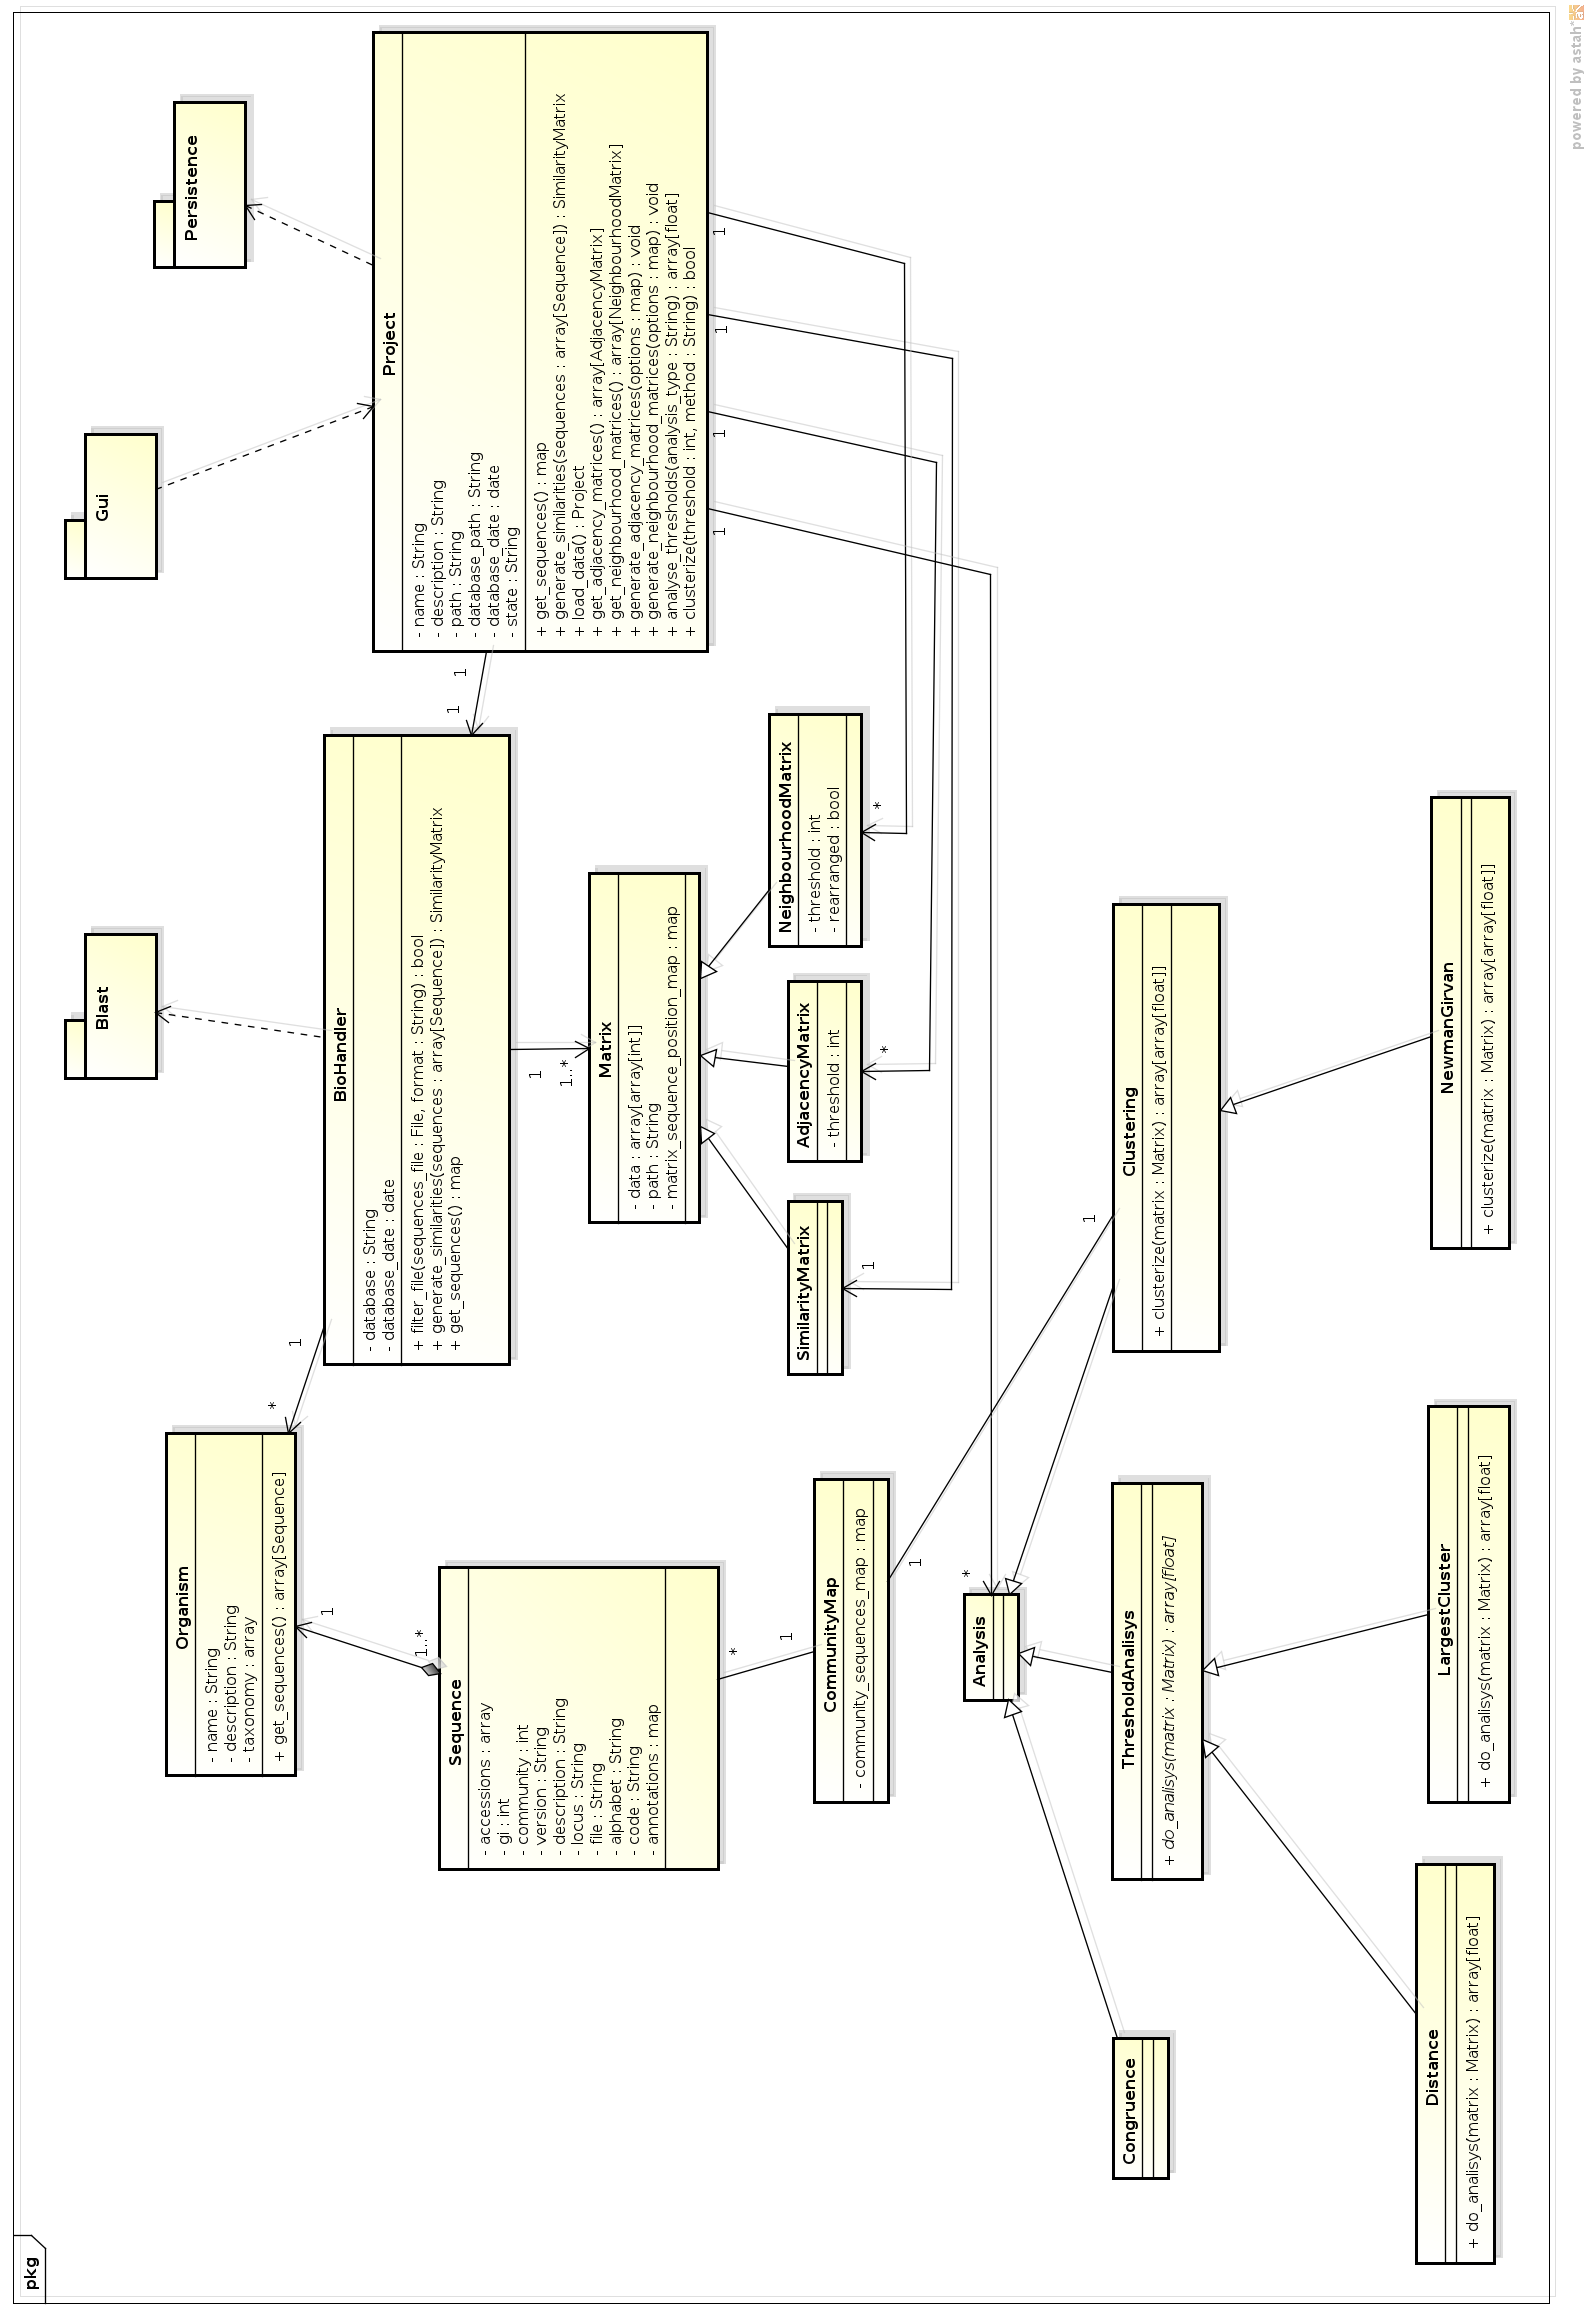
\includegraphics[scale=0.28]{diagrama-classes-completo}
\caption{Diagrama de classes completo do AIAF.}
\label{fig:diagrama-classes-completo}
\end{figure}

\chapter{Diagramas de Sequências}

\begin{figure}
\centering
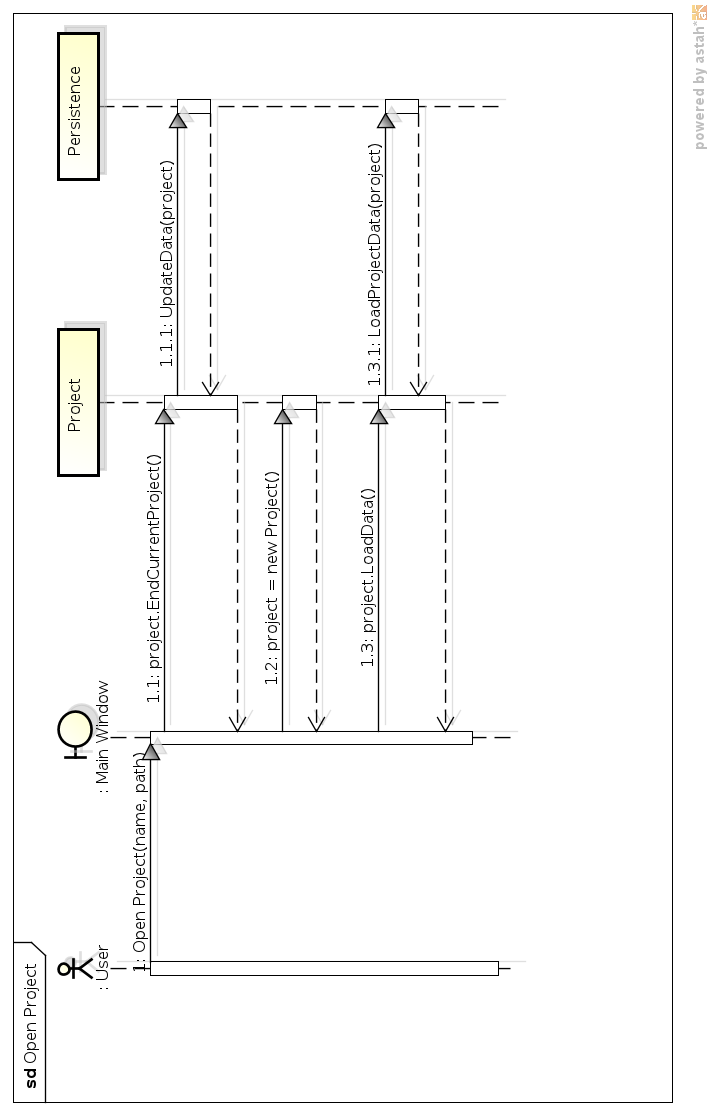
\includegraphics[scale=0.47]{open-project}
\caption{Diagrama de sequências para o caso de uso 2: abrir projeto existente.}
\label{fig:open-project}
\end{figure}

\begin{figure}
\centering
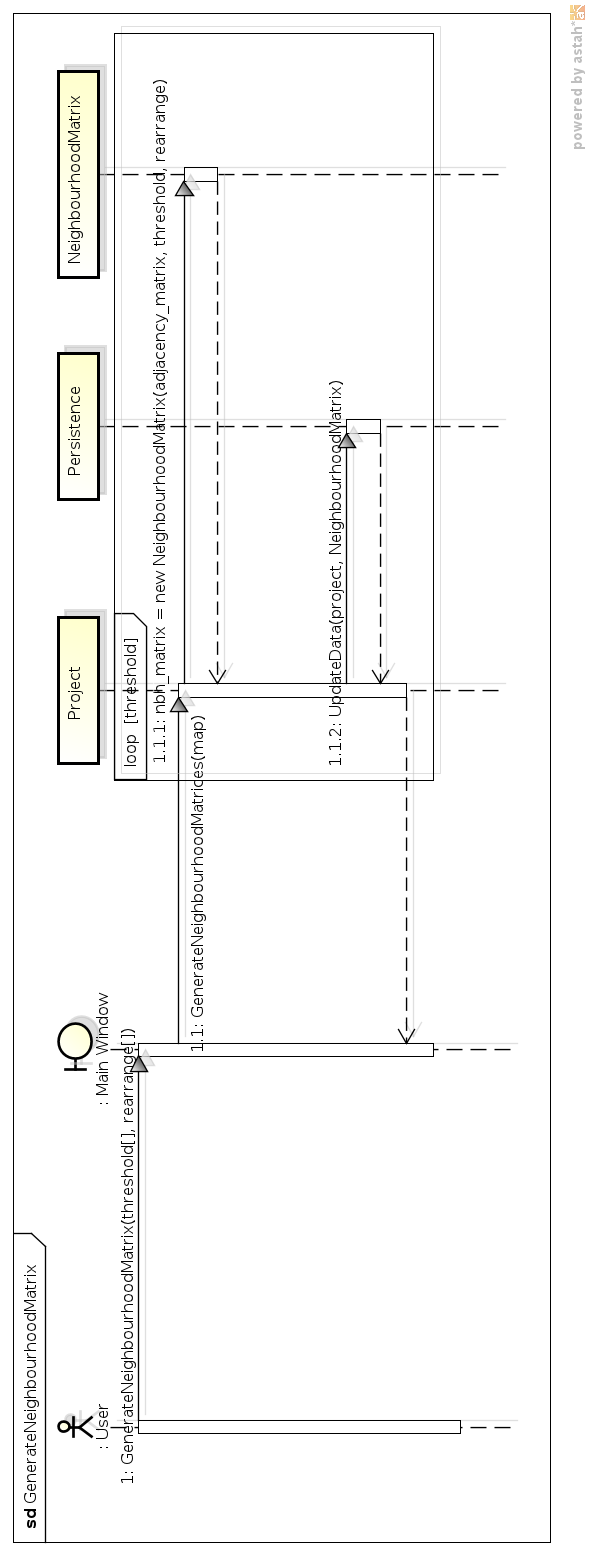
\includegraphics[scale=0.37]{generate-neighbourhood-matrix}
\caption{Diagrama de sequências para o caso de uso 4: gerar matriz de vizinhança de um limiar qualquer.}
\label{fig:generate-neighbourhood-matrix}
\end{figure}

\begin{figure}
\centering
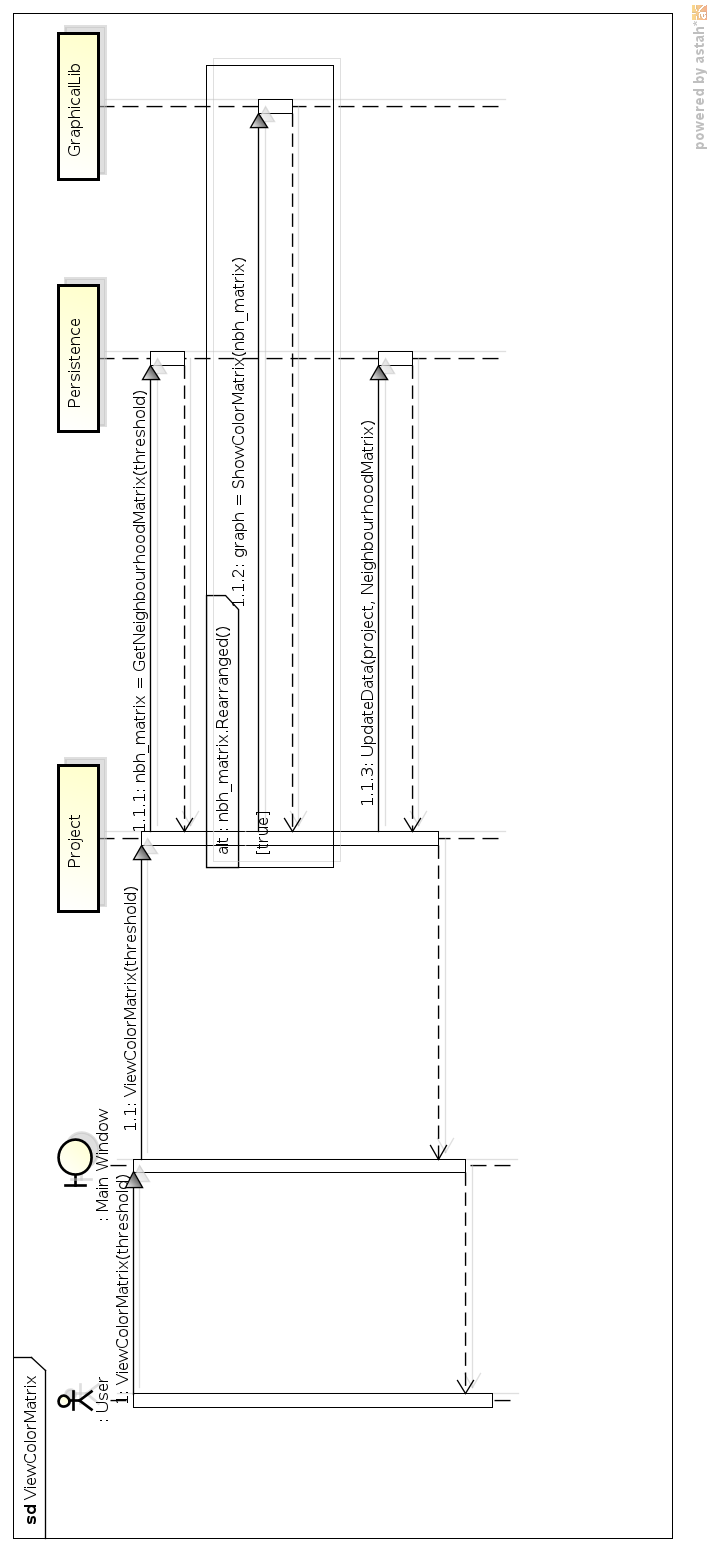
\includegraphics[scale=0.43]{view-color-matrix}
\caption{Diagrama de sequências para o caso de uso 5: visualizar gráfico de matriz de vizinhança qualquer em forma de matriz de cores.}
\label{fig:view-color-matrix}
\end{figure}

\begin{figure}
\centering
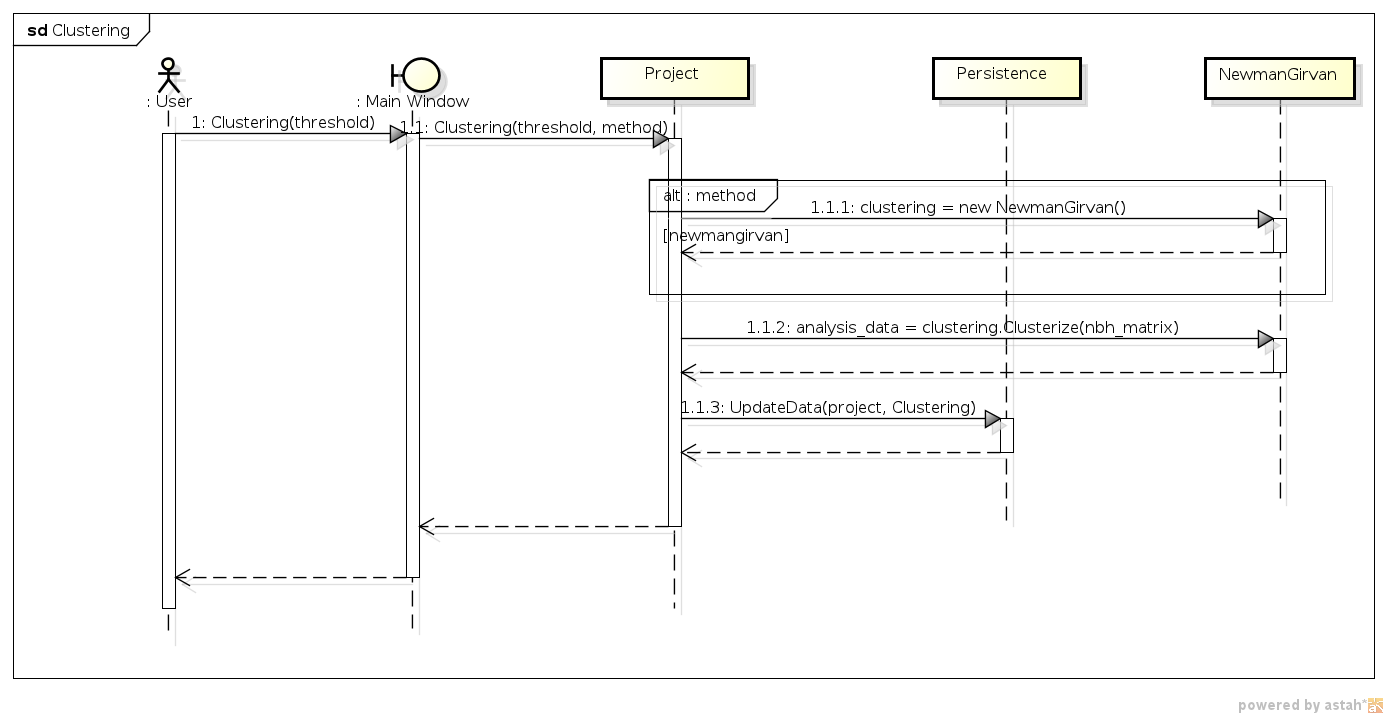
\includegraphics[scale=0.47]{clustering}
\caption{Diagrama de sequências para o caso de uso 7: executar clusterização.}
\label{fig:clustering}
\end{figure}

\begin{figure}
\centering
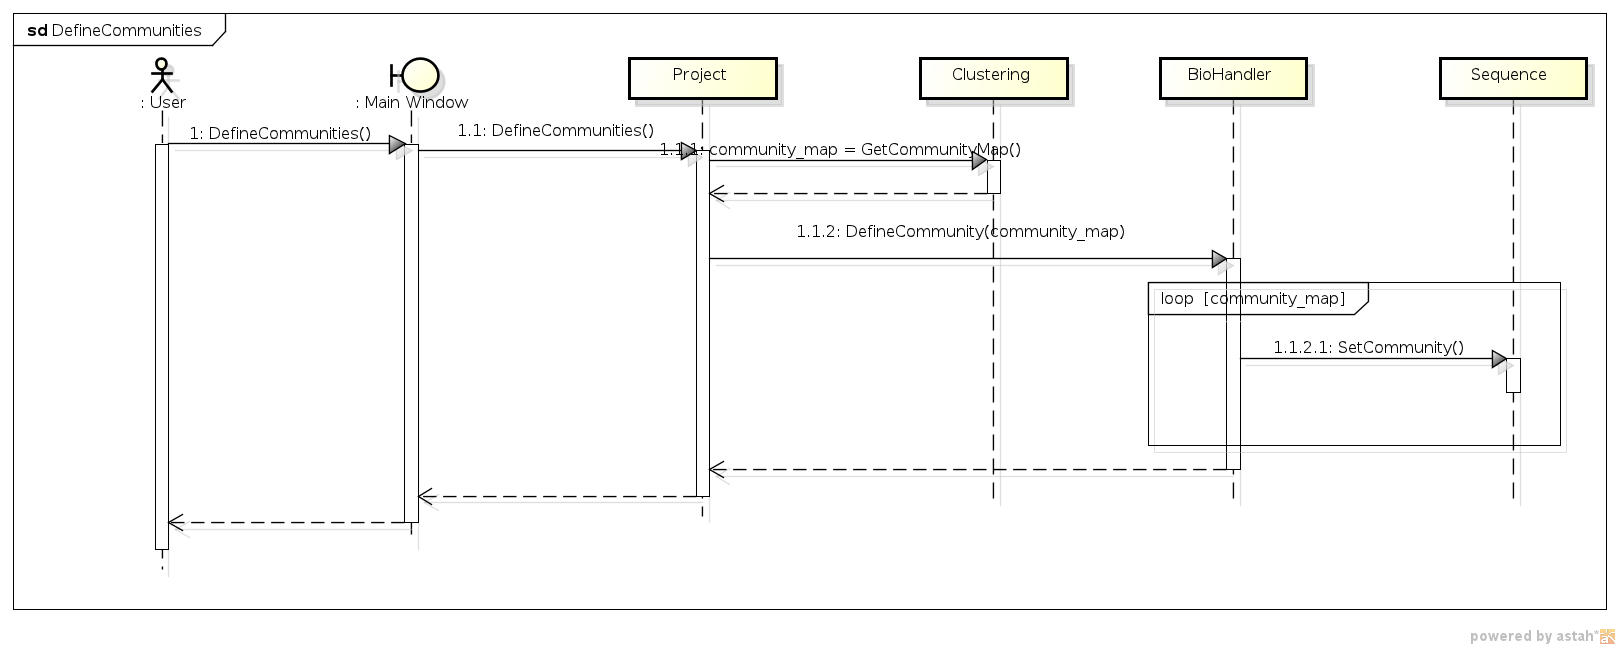
\includegraphics[scale=0.41]{define-communities}
\caption{Diagrama de sequências para o caso de uso 8: definir módulos/comunidades.}
\label{fig:define-communities}
\end{figure}

\begin{figure}
\centering
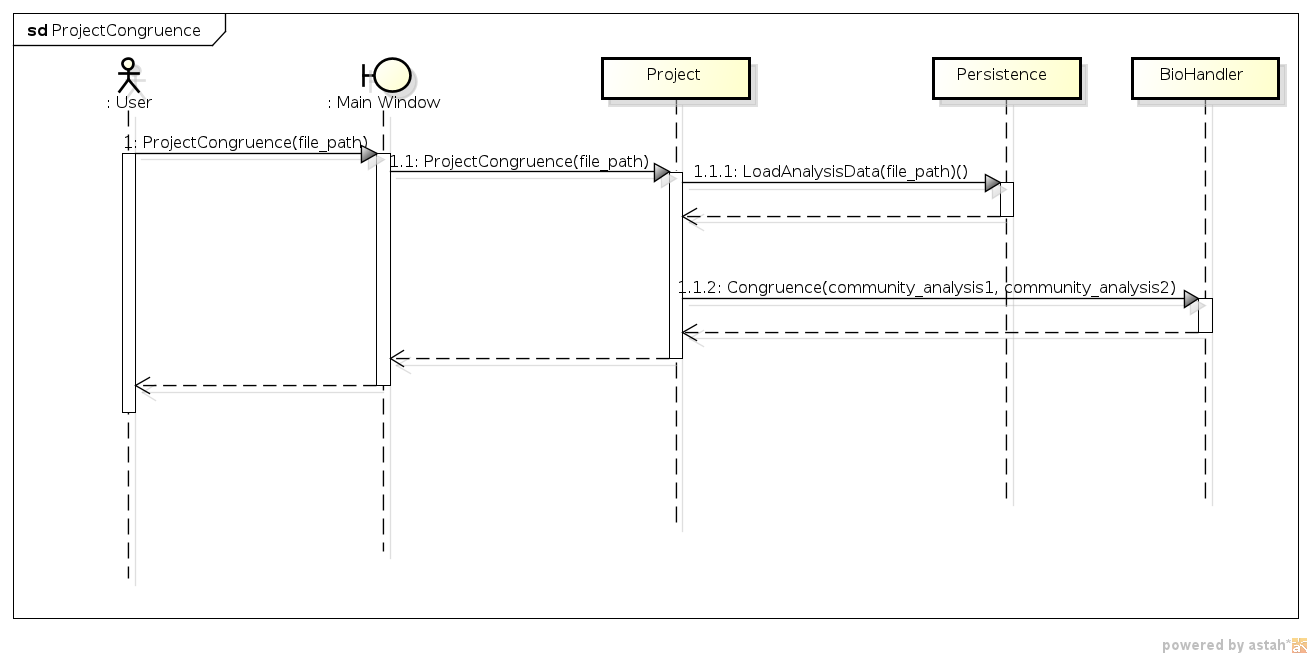
\includegraphics[scale=0.47]{project-congruence}
\caption{Diagrama de sequências para o caso de uso 9: comparar/executar congruência de redes de diferentes projetos.}
\label{fig:project-congruence}
\end{figure}

\begin{figure}
\centering
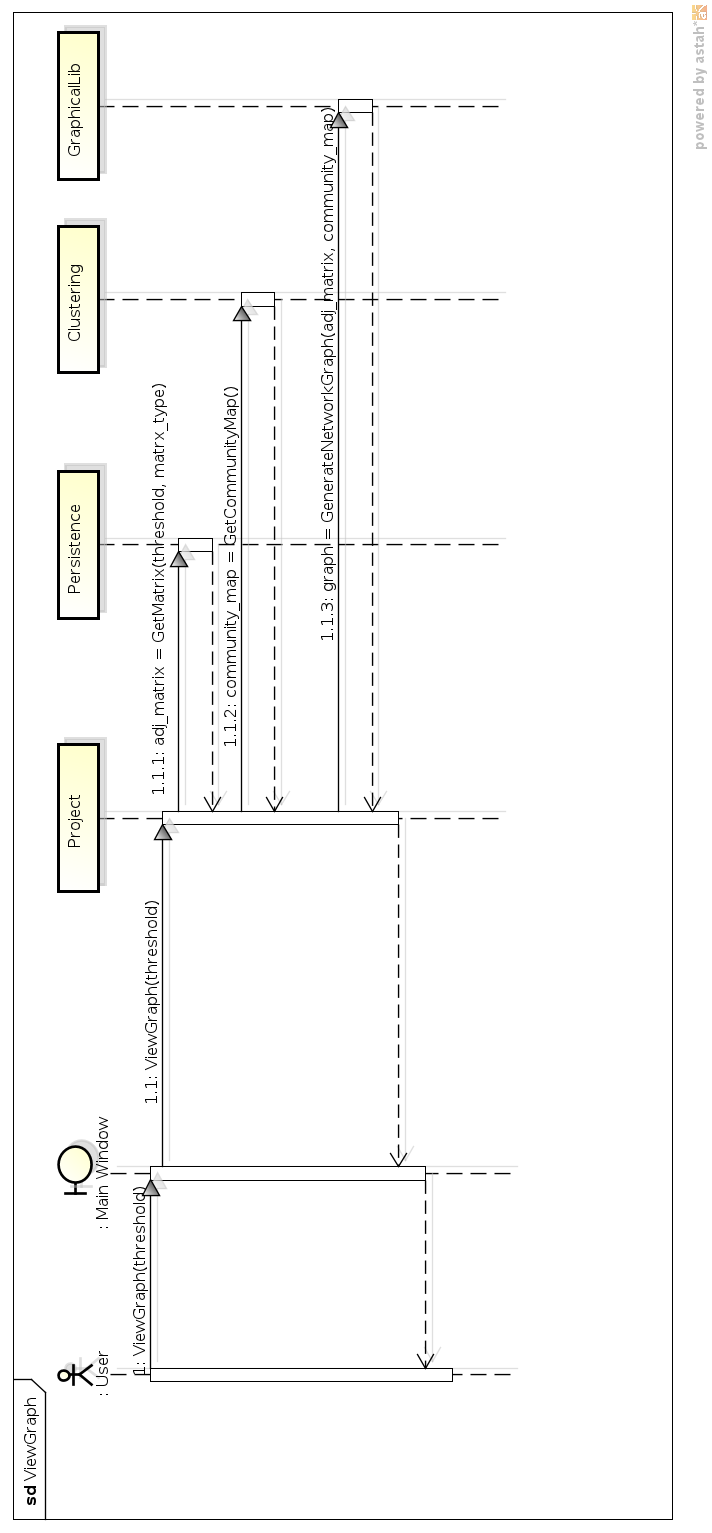
\includegraphics[scale=0.41]{view-graph}
\caption{Diagrama de sequências para o caso de uso 10: visualizar gráfico completo da rede.}
\label{fig:view-graph}
\end{figure}

\begin{figure}
\centering
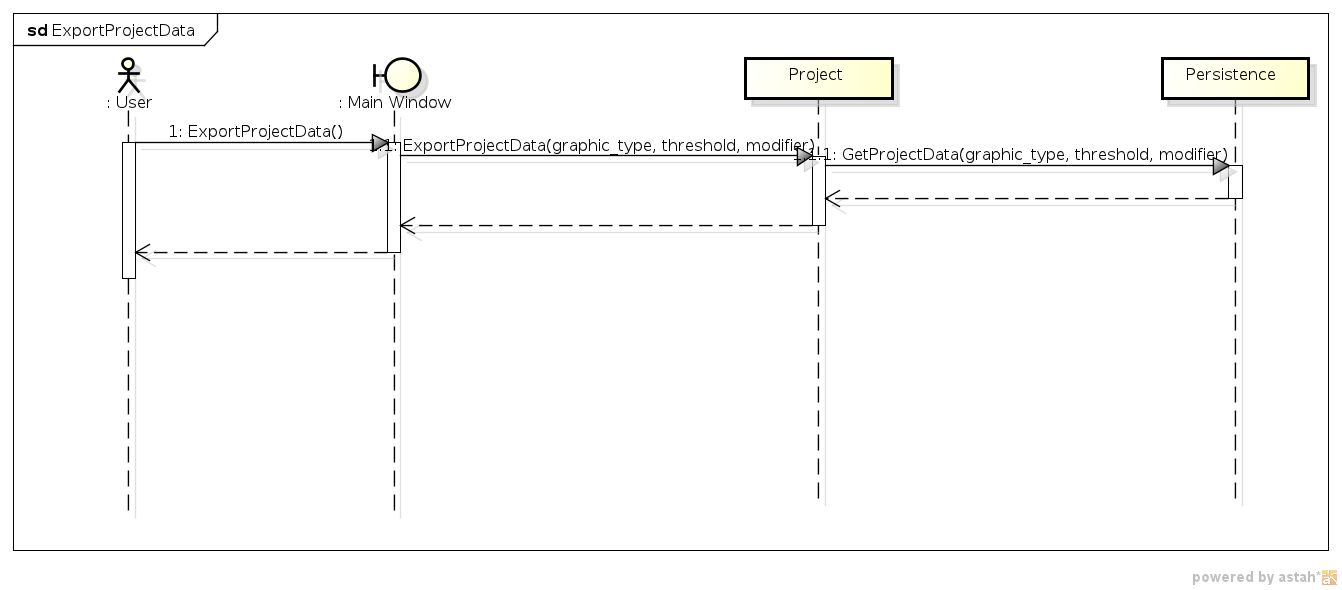
\includegraphics[scale=0.43]{export-project-data}
\caption{Diagrama de sequências para o caso de uso 12: exportar dados do projeto para gráficos.}
\label{fig:export-project-data}
\end{figure}